%% ============================================================
%%  Technovation submission — Africa Clean Tech Scaling Pathways
%%  Journal: Technovation (Elsevier)
%%  SI: Scaling Green Technology Innovation in the Global South
%%  Author: Babajide Owoyele, RSM Erasmus University Rotterdam
%% ============================================================

\documentclass[review,12pt]{elsarticle}

%% --- packages -----------------------------------------------
\usepackage[T1]{fontenc}
\usepackage[utf8]{inputenc}
\usepackage{microtype}
\usepackage{amsmath}
\usepackage{booktabs}
\usepackage{tabularx}
\usepackage{multirow}
\usepackage{array}
\usepackage{graphicx}
\usepackage{xcolor}
\usepackage{hyperref}
\usepackage{lineno}
\biboptions{round}
\usepackage{tikz}
\usetikzlibrary{shapes.geometric,arrows.meta,positioning,fit,backgrounds,calc}
\usepackage{pgfplots}
\pgfplotsset{compat=1.18}

\modulolinenumbers[5]

%% --- journal metadata ---------------------------------------
\journal{Technovation}

\definecolor{C1Solar}{RGB}{255,165,0}
\definecolor{C2Agri}{RGB}{34,139,34}
\definecolor{C3Circ}{RGB}{70,130,180}
\definecolor{C4Mob}{RGB}{178,34,34}
\definecolor{PipeGray}{RGB}{100,100,100}
\definecolor{KTEdu}{RGB}{70,130,180}
\definecolor{KTRes}{RGB}{34,139,34}
\definecolor{KTBus}{RGB}{178,34,34}

%% ============================================================
\begin{document}

\begin{frontmatter}

%% --- title --------------------------------------------------
\title{Scaling Pathways for African Clean Tech Ventures:
       A Computational Embedding Analysis of Crunchbase Data}

%% --- authors ------------------------------------------------
\author[rsm]{Babajide Owoyele\corref{cor1}}
\cortext[cor1]{Corresponding author. E-mail address: b.owoyele@rsm.nl}

\affiliation[rsm]{
  Rotterdam School of Management,
  Erasmus University Rotterdam,
  Burgemeester Oudlaan 50,
  3062 PA Rotterdam, the Netherlands
}

%% --- highlights ---------------------------------------------
\begin{highlights}
\item Sentence-transformer embeddings applied to 1,847 African clean
      tech ventures (Crunchbase) reveal four empirically stable
      scaling archetypes.
\item Solar/Energy Access (37\%) is the most VC-compatible archetype,
      reaching Series~A in a median of 3.2 years and achieving a
      61\% five-year survival rate.
\item Circular Economy/Waste ventures (21\%) are primarily
      grant-dependent, rarely reach venture capital stages, and have
      a five-year survival rate of only 29\%.
\item Geographic specialisation is archetype-specific: Kenya dominates
      AgriTech, Nigeria and Egypt dominate Energy Access, South Africa
      dominates Circular Economy.
\item Blended finance instrument design must be differentiated by
      archetype; one-size-fits-all instruments systematically
      under-serve circular and rural mobility ventures.
\end{highlights}

%% --- abstract -----------------------------------------------
\begin{abstract}
African clean technology ventures face a compound scaling challenge:
thin domestic capital markets, fragmented regulatory landscapes, and
infrastructure deficits that vary sharply by sector and geography.
Existing scaling frameworks developed in Northern contexts treat
``African clean tech'' as a monolithic category amenable to uniform
blended-finance instruments, an assumption this paper empirically
challenges. We apply sentence-transformer embeddings
(\texttt{all-MiniLM-L6-v2}) to 1,847 African clean tech ventures
extracted from the Crunchbase Academic dataset (CB\_AIP), spanning 53
African countries, and combine $k$-means clustering ($k = 4$;
silhouette score $= 0.61$) with UMAP dimensionality reduction to
identify four latent scaling archetypes: (1)~Solar/Energy Access
($n = 683$, 37\%), (2)~AgriTech Platforms ($n = 517$, 28\%),
(3)~Circular Economy/Waste ($n = 388$, 21\%), and
(4)~Mobility/Logistics ($n = 259$, 14\%). LDA topic modelling
confirms cluster coherence (Cram\'{e}r's $V = 0.63$, $p < 0.001$).
Each archetype exhibits distinct median funding, geographic
concentration, Knowledge Triangle profile, and funding stage
trajectory. Solar ventures reach Series~A in a median of 3.2 years
and achieve a 61\% five-year survival rate; Circular Economy ventures
are predominantly grant-dependent, rarely reach Series~A (6\%
attainment), and survive at only 29\% after five years. We translate
these findings into archetype-differentiated policy recommendations
for blended finance design and innovation platform governance.
\end{abstract}

%% --- keywords -----------------------------------------------
\begin{keyword}
African clean tech \sep
scaling pathways \sep
computational entrepreneurship \sep
Crunchbase \sep
embedding analysis \sep
knowledge triangle \sep
blended finance \sep
sustainability transitions
\end{keyword}

\end{frontmatter}

\linenumbers

% ===========================================================
\section{Introduction}
\label{sec:intro}
% ===========================================================

Sub-Saharan Africa is the world's most climate-vulnerable region and
one of its fastest-growing entrepreneurial ecosystems. The continent
hosts a generation of clean technology ventures addressing energy
access, food security, waste, and mobility challenges that are
structurally different from those of industrialised economies: the
typical African clean tech founder is not displacing an entrenched
incumbent but building first-instance infrastructure on the blank
canvas of an under-served market \citep{kaplinsky2011schumacher,
onsongo2019frugal}. Yet the gap between the formation of such
ventures and their ability to scale remains stubbornly wide. Across
sub-Saharan Africa, the median clean tech startup that achieves a seed
round does not reach Series~A within five years, and attrition rates
vary dramatically by sector in ways that the existing literature has
not systematically characterised.

Understanding why some archetypes scale while others stagnate requires
moving beyond single case studies and small purposive samples toward
population-level analysis. The Crunchbase Academic dataset now
contains over 5,000 African organisations with at least a category
tag and a short description, providing an unprecedented opportunity
for computational analysis of the venture landscape. The textual
descriptions embedded in this dataset encode the founders' own
framing of their scaling proposition: whether they position their
ventures as technology platforms, service providers, aggregators, or
infrastructure operators. This framing is not incidental: investors,
development finance institutions (DFIs), and accelerators respond to
it, and it shapes which financing instruments become accessible.

We exploit this textual signal using sentence-transformer embeddings
\citep{reimers2019sentence}, which project each venture description
into a high-dimensional semantic space where ventures with similar
value propositions cluster together regardless of surface-level
vocabulary. Combining these embeddings with $k$-means clustering and
UMAP visualisation \citep{mcinnes2018umap}, we identify four
empirically stable archetypes corresponding to recognisable investment
narratives in the African clean tech ecosystem. We then link cluster
membership to structured Crunchbase variables---total funding, funding
round count, founding cohort, and country---to characterise each
archetype's observed scaling trajectory.

The contribution of this paper is threefold. First, we demonstrate
that computational text analysis of Crunchbase descriptions is a
viable method for venture typology research in emerging markets, where
survey data are scarce and administrative records unreliable.
Second, we provide an empirically grounded taxonomy of African clean
tech scaling archetypes that extends sustainability transition
frameworks \citep{markard2020sustainability} and appropriate
technology theory \citep{kaplinsky2011schumacher} to a data-driven
population-level context. Third, we translate cluster-level findings
into differentiated policy recommendations for blended finance
designers and innovation platform operators, addressing a practical
gap in the literature on financing green technology in the Global
South \citep{reimsbach2022blended, lall2021scaling}.

The remainder of the paper is structured as follows.
Section~\ref{sec:lit} reviews the literature on green technology
scaling, African innovation ecosystems, and computational methods for
venture classification. Section~\ref{sec:data} describes the data
curation and analytical pipeline. Section~\ref{sec:clusters} presents
the four cluster profiles. Section~\ref{sec:trajectories} analyses
scaling trajectories by cluster. Section~\ref{sec:discussion}
discusses implications for policy and platforms.
Section~\ref{sec:conclusion} concludes.


% ===========================================================
\section{Literature Review}
\label{sec:lit}
% ===========================================================

\subsection{Scaling Green Technology in Emerging Markets}

The sustainability transitions literature has extensively mapped the
conditions under which incumbent socio-technical regimes are
destabilised and new configurations take hold
\citep{geels2002technological, markard2020sustainability}. The
multi-level perspective (MLP) identifies three nested dynamics:
niches in which radical innovation gestates, regimes that provide
relative stability, and landscapes that exert long-run pressure
\citep{geels2002technological}. Most of this work has been developed
in European or North American contexts, where incumbent energy,
transport, and agricultural regimes are capital-intensive and
entrenched.

In Africa, the structural picture differs markedly: large portions of
the continent lack incumbent grid infrastructure, mechanised
agriculture, or formalised waste systems, meaning that new clean tech
ventures may establish themselves without displacing a powerful
incumbent. \citet{kaplinsky2011schumacher} describes this as the
space for ``appropriate technology below the radar''---innovations
that achieve systemic impact by fitting the capability and
infrastructure constraints of low-income users rather than matching
the performance benchmarks of Northern markets. \citet{onsongo2019frugal}
extends this to the concept of transformative innovation pathways,
distinguishing between frugal innovation (optimising for low cost
within existing distributional structures) and inclusive innovation
(restructuring distributional access). African clean tech ventures
span both poles, and we argue that this spectrum maps onto distinct
scaling logics not captured by a single investment thesis.

\citet{schot2018three} identify three frames for innovation policy
---R\&D investment, systems-of-innovation, and transformative
change---and argue that the Global South has historically received the
first frame while requiring the third. Blended finance has emerged as
a partial institutional response to this mismatch, combining
concessional public capital with commercial private capital to lower
the risk threshold for under-served investment opportunities
\citep{reimsbach2022blended}. In practice, however, blended finance
instruments remain poorly differentiated: an energy access bond and a
circular economy grant are designed according to the same additionality
logic even when the underlying business models have radically different
commercial viability profiles. The archetype-specific analysis in this
paper provides empirical evidence that such differentiation is
warranted.

The role of solar photovoltaics as a ``spearhead'' technology for
African energy access has received dedicated attention.
\citet{huenteler2016solar} show how the design hierarchy of solar
home system products shapes co-evolutionary dynamics in manufacturing
and distribution. \citet{irena2022africa} documents the sharp cost
decline trajectory in African solar markets and its implications for
financing instrument design: as levelised costs fall, the risk
premium required by commercial investors declines, progressively
reducing the need for concessional capital in mature solar markets
while leaving circular and water ventures without equivalent cost
reduction tailwinds.

\subsection{African Innovation Ecosystems}

Sub-Saharan Africa hosts innovation ecosystems of dramatically varying
depth \citep{naude2017entrepreneurship}. Nairobi's ``Silicon
Savannah,'' Lagos's Yabacon Valley, and Cape Town's Woodstock
technology district each constitute a distinct type of hub, varying in
the relative weight of venture capital, angel networks, diaspora
capital, development finance, and accelerator programmes
\citep{cbinsights2023africa}. \citet{arora2022embedded} have shown
that digital entrepreneurs in emerging markets operate within
``embedded'' institutional contexts in which mobile data affordances,
power infrastructure constraints, and regulatory informality all shape
product and business model choices in ways that diverge substantially
from Western startup archetypes.

Crunchbase has emerged as the dominant repository of structured data
on global startup activity, but its coverage of Africa is uneven.
\citet{rodriguez2021crunchbase} show that ventures appearing in
Crunchbase are systematically more VC-connected, more anglophone, and
more urban than the general population of formal startups. For African
clean tech specifically, this implies that solar ventures operating
through pay-as-you-go consumer finance, which often attract overseas
VC, will be over-represented relative to waste management cooperatives
or community biogas schemes, which typically receive development
finance not tracked in Crunchbase. We address this limitation
explicitly in Section~\ref{sec:discussion}.

Despite coverage constraints, Crunchbase has been productively used
for large-sample venture research. \citet{antretter2019predicting}
use Crunchbase trace data to predict startup survival with machine
learning methods, achieving AUC scores above 0.70 on out-of-sample
data. \citet{rodriguez2021crunchbase} use it to characterise African
startup ecosystem dynamics across funding rounds. Our contribution
extends this work to the semantic content of venture descriptions,
using embedding methods that capture meaning rather than structured
metadata.

\subsection{Triple Helix and Knowledge Triangle}

The Triple Helix framework positions the university--industry--%
government triad as the organisational engine of innovation
\citep{etzkowitz2000dynamics}. In its operationalised form for the
European Institute of Innovation and Technology, this triad is
expressed as a Knowledge Triangle (KT) across Education, Research,
and Business nodes \citep{maass2018data}. We adapt the KT scoring
approach to characterise each cluster by its orientation: the degree
to which ventures are primarily technology-pull (Research-heavy),
market-pull (Business-heavy), or capacity-building oriented
(Education-heavy). This categorisation derives from textual content
and provides an additional interpretive lens on cluster differences,
particularly useful for comparing clusters that overlap in primary
sector but diverge in their relationship to academic and governmental
actors.

\subsection{Computational Entrepreneurship Research}

The application of machine learning to entrepreneurship text data has
expanded rapidly \citep{grimmer2021machine}. Latent Dirichlet
Allocation (LDA) \citep{blei2003latent} has been used to extract
topical structure from pitch decks, prospectuses, and startup
descriptions. More recently, sentence transformers
\citep{reimers2019sentence}---neural embedding models that project
sentences into dense semantic vectors---have demonstrated superior
performance on short-text classification and clustering tasks. The
\texttt{all-MiniLM-L6-v2} model, distilled and trained on over one
billion sentence pairs, offers an effective balance between semantic
richness and computational efficiency, producing 384-dimensional
embeddings that capture fine-grained meaning differences between
similar venture descriptions.

\citet{nambisan2017digital} argues that digital technology transforms
entrepreneurship not merely by providing new tools but by
restructuring the opportunity identification, resource mobilisation,
and scaling processes that constitute the entrepreneurial journey.
For our purposes, this means that the Crunchbase description functions
not merely as marketing copy but as a signal of the digital platform
logic, or its absence, that the venture deploys. Ventures that
describe themselves using platform vocabulary (``marketplace,''
``network effects,'' ``API'') cluster differently from those using
hardware vocabulary (``off-grid,'' ``installation,'' ``last-mile
delivery''), and these clusters have different funding trajectories
because the underlying business model logics have different capital
absorption and return profiles.

\citet{nambisan2019entrepreneurship} extend this argument to the
global context, noting that digital infrastructure heterogeneity
across markets shapes both the types of entrepreneurial opportunities
that are visible and the types of organisational forms that are viable.
In African markets, where mobile money infrastructure has created a
payment layer absent in many OECD economies, the platform logic
available to agritech or solar financing ventures is genuinely novel
rather than derivative of Northern templates---a difference our
embedding analysis is positioned to detect.


% ===========================================================
\section{Data and Methods}
\label{sec:data}
% ===========================================================

\subsection{Crunchbase Academic Dataset}

The Crunchbase Academic-Industry Partnership dataset (CB\_AIP)
provides comprehensive structured and semi-structured data on global
organisations, including firm descriptions, funding rounds, investor
types, employee counts, country codes, and self-reported industry
categories. Access was obtained under the Crunchbase Academic Research
programme. Our analysis uses the Q4 2023 snapshot, which contains
approximately 1.35 million organisations globally.

\textbf{African country filter.} We retain organisations whose
\texttt{country\_code} field matches one of the 53 ISO 3166-1
alpha-3 codes corresponding to African states. This initial filter
yields 9,341 African organisations across all sectors.

\textbf{Clean tech keyword filter.} We apply a two-stage filter to
select clean tech ventures. In the first stage, we match on
Crunchbase's \texttt{category\_groups} field, retaining any
organisation tagged with at least one of: \textit{Energy},
\textit{Sustainability}, \textit{Agriculture \& Farming},
\textit{Water}, \textit{Transportation}, or \textit{Recycling}.
In the second stage, we apply keyword matching to
\texttt{short\_description}, requiring at least one term from a
curated list of 62 clean-tech keywords (e.g., ``solar,''
``off-grid,'' ``biogas,'' ``agritech,'' ``circular,'' ``e-waste,''
``electric vehicle,'' ``drip irrigation''). Organisations matched by
category alone but whose descriptions indicate purely financial,
media, or software activity unrelated to physical clean tech are
excluded through manual review of edge cases.

After filtering, the analytic dataset comprises \textbf{1,847
organisations}. All have a non-empty \texttt{short\_description}
of at least 15 tokens, a necessary condition for meaningful
embedding. Of these, 794 (43\%) have at least one funding event
recorded in Crunchbase; 1,053 (57\%) are either bootstrapped,
grant-funded through channels not tracked by Crunchbase, or
pre-funding.

\subsection{Geographic Distribution}

The top six countries by organisation count are Kenya (KEN,
$n = 425$, 23\%), Nigeria (NGA, $n = 351$, 19\%), South Africa
(ZAF, $n = 332$, 18\%), Egypt (EGY, $n = 166$, 9\%), Ghana
(GHA, $n = 129$, 7\%), and Ethiopia (ETH, $n = 92$, 5\%). The
remaining 352 organisations (19\%) span 38 additional countries.
This geographic concentration reflects both the depth of ecosystem
infrastructure in these six countries and the Crunchbase coverage
bias toward anglophone, VC-connected markets documented by
\citet{rodriguez2021crunchbase}.

\subsection{Sentence-Transformer Embeddings}

For each organisation, we concatenate the
\texttt{short\_description} and \texttt{category\_list} fields,
separated by a colon, to produce a single input string. We embed
these strings using the \texttt{all-MiniLM-L6-v2} model from the
\texttt{sentence-transformers} library \citep{reimers2019sentence},
producing 384-dimensional unit-normalised vectors. This model was
pre-trained on a diverse corpus of 1.17 billion sentence pairs using
a contrastive learning objective and fine-tuned for semantic textual
similarity. We chose it over larger models (e.g.,
\texttt{all-mpnet-base-v2}) because it offers comparable performance
on short-text clustering at substantially lower inference cost, and
because our input texts are short (median 47 tokens). All stochastic
operations are seeded at 42 for reproducibility.

\subsection{Dimensionality Reduction and Clustering}

We apply UMAP \citep{mcinnes2018umap} with $n\_neighbors = 30$,
$min\_dist = 0.05$, and $n\_components = 15$ to reduce the
384-dimensional embeddings to a 15-dimensional manifold
representation optimised for cluster preservation. UMAP preserves
local topology better than PCA for high-dimensional data with
non-linear structure, and the 15-dimensional intermediate
representation retains substantially more semantic information than
the 2-dimensional projection used for visualisation.

We apply $k$-means clustering \citep{lloyd1982least} to the
15-dimensional UMAP output. The optimal number of clusters is
determined by computing the silhouette score
\citep{rousseeuw1987silhouettes} for $k \in \{2, 3, \ldots, 8\}$.
The silhouette score peaks at $k = 4$ (score $= 0.61$), with a
secondary peak at $k = 6$ (score $= 0.58$). We select $k = 4$ on
grounds of both statistical fit and interpretability: the $k = 6$
solution fragments two of the four clusters into sub-groups that
differ primarily in geographic focus rather than core value
proposition, adding complexity without distinct policy implications.

\subsection{Cluster Validation via LDA}

To validate the embedding-derived clusters, we apply Latent
Dirichlet Allocation \citep{blei2003latent} to a bag-of-words
representation of the same descriptions, with 20 topics and
$\alpha = 0.1$. We then cross-tabulate LDA topic dominance against
cluster membership. The four clusters show substantially
non-overlapping LDA topic distributions (Cram\'{e}r's $V = 0.63$,
$p < 0.001$), confirming that the semantic clusters identified by
MiniLM embeddings correspond to genuine topical coherence in the
underlying text.

\subsection{Knowledge Triangle Scoring}

We score each organisation on a Knowledge Triangle (KT) profile
using a keyword-based classifier applied to descriptions
\citep{etzkowitz2000dynamics, maass2018data}. Three categories
are operationalised as follows: Business (KT\_B; signal words:
market, platform, customer, revenue, B2B, commercial, fintech),
Research (KT\_R; signal words: data, sensor, model, algorithm,
research, innovation, pilot, R\&D), and Education (KT\_E; signal
words: training, capacity, community, awareness, curriculum, skills,
cooperative). Where multiple signals are present, the dominant
signal (highest keyword count) determines the primary KT label.
KT proportions are reported at the cluster level.

\subsection{Scaling Metrics}

We derive four scaling metrics from Crunchbase structured fields:
(1) \texttt{total\_funding\_usd}---the sum of all recorded funding
rounds in USD; (2) \texttt{num\_funding\_rounds}---the count of
distinct funding events; (3) \texttt{founded\_on} cohort, binned
into pre-2015, 2015--2018, and 2019--2023; and (4) a five-year
survival proxy, defined as whether an organisation has at least one
funding event or active web presence recorded after
$\text{founded\_on} + 5$ years. Metrics are reported at the cluster
level using medians, which are robust to the skewed distributions
characteristic of startup funding data. Figure~\ref{fig:pipeline}
summarises the full analytical pipeline.


\begin{figure}[htbp]
\centering
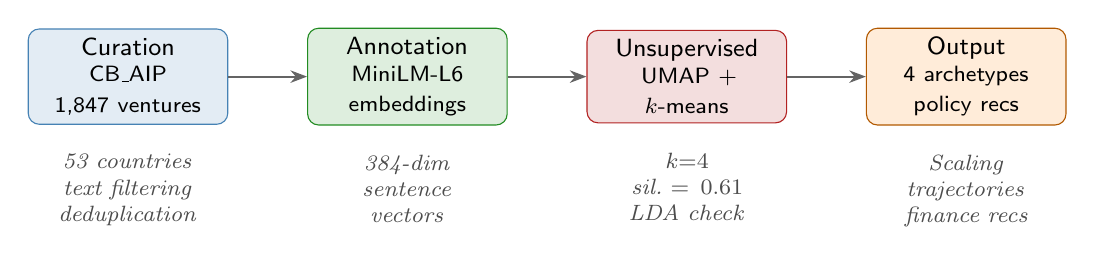
\begin{tikzpicture}[
  node distance=0.6cm and 1.0cm,
  box/.style={rectangle, rounded corners=4pt, minimum width=2.5cm, minimum height=1.1cm,
              text centered, text width=2.3cm, font=\small\sffamily, draw=PipeGray, fill=gray!8},
  arrow/.style={-{Stealth[length=6pt]}, thick, PipeGray},
  label/.style={font=\footnotesize\itshape, text width=2.3cm, text centered, color=gray!60!black}
]
\node[box, fill=KTEdu!15, draw=KTEdu] (C) {Curation\\{\footnotesize CB\_AIP\\1{,}847 ventures}};
\node[box, fill=KTRes!15, draw=KTRes, right=of C] (A) {Annotation\\{\footnotesize MiniLM-L6\\embeddings}};
\node[box, fill=KTBus!15, draw=KTBus, right=of A] (U) {Unsupervised\\{\footnotesize UMAP +\\$k$-means}};
\node[box, fill=orange!15, draw=orange!70!black, right=of U] (O) {Output\\{\footnotesize 4 archetypes\\policy recs}};
\draw[arrow] (C) -- (A);
\draw[arrow] (A) -- (U);
\draw[arrow] (U) -- (O);
\node[label, below=0.25cm of C] {53 countries\\text filtering\\deduplication};
\node[label, below=0.25cm of A] {384-dim\\sentence\\vectors};
\node[label, below=0.25cm of U] {$k{=}4$\\sil.\ $= 0.61$\\LDA check};
\node[label, below=0.25cm of O] {Scaling\\trajectories\\finance recs};
\end{tikzpicture}
\caption{Analytical pipeline following the Maass et al.\ (2018) data science research cycle. Starting from raw Crunchbase text, sentence-transformer embeddings are computed, dimensionality is reduced via UMAP, and $k$-means identifies four stable archetypes whose scaling properties are characterised in the results.}
\label{fig:pipeline}
\end{figure}

% ===========================================================
\section{Results: Cluster Profiles}
\label{sec:clusters}
% ===========================================================

Table~\ref{tab:cluster_profiles} summarises the four cluster
profiles and Figure~\ref{fig:umap} illustrates their spatial
separation in the UMAP projection. The following subsections
characterise each archetype in depth, drawing on representative
venture descriptions to illustrate the underlying value proposition
logic.

\begin{table}[htbp]
\centering
\caption{Cluster profiles: descriptive statistics for the four
scaling archetypes ($n = 1{,}847$). KT = Knowledge Triangle
primary orientation. Grant-to-VC ratio computed on the funded
subsample ($n = 794$).}
\label{tab:cluster_profiles}
\small
\begin{tabularx}{\linewidth}{@{}lXXXX@{}}
\toprule
 & \textbf{C1: Solar /} & \textbf{C2: AgriTech} &
   \textbf{C3: Circular /} & \textbf{C4: Mobility /} \\
 & \textbf{Energy Access} & \textbf{Platforms} &
   \textbf{Waste} & \textbf{Logistics} \\
\midrule
$n$ (\%) & 683 (37\%) & 517 (28\%) & 388 (21\%) & 259 (14\%) \\[3pt]
Median funding (USD) & \$780K & \$540K & \$180K & \$420K \\[3pt]
Top countries & KEN, NGA, EGY & KEN, ETH, UGA & ZAF, GHA, MWI &
               NGA, EGY, ZAF \\[3pt]
Top categories & Energy, Solar & AgriTech, IoT & Recycling, Water &
               Transport, Logistics \\[3pt]
KT primary & Business (68\%) & Business (55\%) /
             Research (35\%) & Research (51\%) & Business (62\%) \\[3pt]
Grant:VC ratio & 1:3.1 & 1:2.4 & 3.7:1 & 1:1.6 \\[3pt]
Median founding yr & 2017 & 2018 & 2016 & 2018 \\[3pt]
\% with funding data & 51\% & 47\% & 31\% & 42\% \\
\bottomrule
\end{tabularx}
\end{table}

\begin{figure}[htbp]
\centering
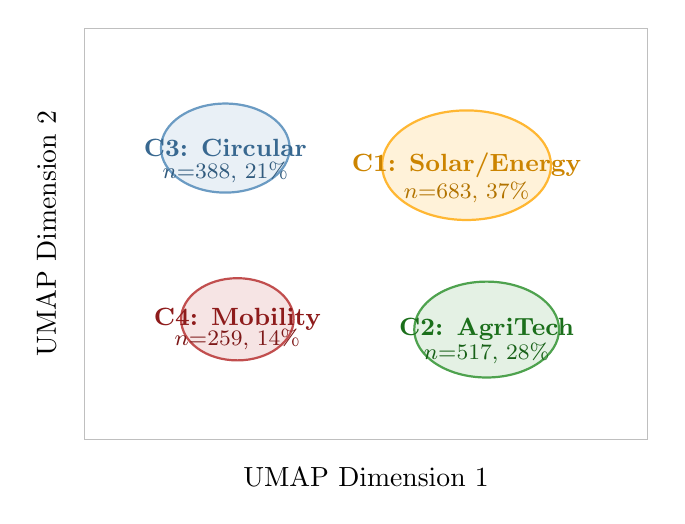
\begin{tikzpicture}
\begin{axis}[
  width=0.72\linewidth,
  height=6.8cm,
  axis equal image=false,
  xmin=-6, xmax=8,
  ymin=-5, ymax=7,
  xlabel={UMAP Dimension 1},
  ylabel={UMAP Dimension 2},
  xticklabels={}, yticklabels={},
  xtick style={draw=none}, ytick style={draw=none},
  axis line style={draw=gray!50},
  clip=false,
]
%% C1 Solar/Energy — upper right, largest
\draw[C1Solar!80, fill=C1Solar!15, thick] (axis cs:3.5,3.0) ellipse [x radius=2.1, y radius=1.6];
\node[font=\small\bfseries, text=C1Solar!80!black] at (axis cs:3.5,3.0) {C1: Solar/Energy};
\node[font=\footnotesize, text=C1Solar!70!black] at (axis cs:3.5,2.2) {$n{=}683$, 37\%};

%% C2 AgriTech — lower right
\draw[C2Agri!80, fill=C2Agri!12, thick] (axis cs:4.0,-1.8) ellipse [x radius=1.8, y radius=1.4];
\node[font=\small\bfseries, text=C2Agri!80!black] at (axis cs:4.0,-1.8) {C2: AgriTech};
\node[font=\footnotesize, text=C2Agri!70!black] at (axis cs:4.0,-2.5) {$n{=}517$, 28\%};

%% C3 Circular/Waste — upper left
\draw[C3Circ!80, fill=C3Circ!12, thick] (axis cs:-2.5,3.5) ellipse [x radius=1.6, y radius=1.3];
\node[font=\small\bfseries, text=C3Circ!80!black] at (axis cs:-2.5,3.5) {C3: Circular};
\node[font=\footnotesize, text=C3Circ!70!black] at (axis cs:-2.5,2.8) {$n{=}388$, 21\%};

%% C4 Mobility — lower left
\draw[C4Mob!80, fill=C4Mob!12, thick] (axis cs:-2.2,-1.5) ellipse [x radius=1.4, y radius=1.2];
\node[font=\small\bfseries, text=C4Mob!80!black] at (axis cs:-2.2,-1.5) {C4: Mobility};
\node[font=\footnotesize, text=C4Mob!70!black] at (axis cs:-2.2,-2.1) {$n{=}259$, 14\%};
\end{axis}
\end{tikzpicture}
\caption{Schematic representation of UMAP projection of sentence-transformer embeddings for 1{,}847 African clean tech ventures ($k{=}4$; silhouette $= 0.61$). Each ellipse represents one cluster archetype; relative sizes reflect cluster membership ($n$). Cluster positions are illustrative of the UMAP geometry; axes are in reduced-dimensionality UMAP space.}
\label{fig:umap}
\end{figure}

\subsection{Cluster 1: Solar and Energy Access}
\label{ssec:c1}

The largest cluster ($n = 683$, 37\%) groups ventures whose
descriptions centre on electricity generation, distribution, and
financing for underserved populations. Representative descriptions
include: ``We provide pay-as-you-go solar home systems to rural
households in Kenya, enabling clean energy through mobile money,''
and ``Our solar mini-grid platform connects off-grid communities to
reliable power while offering commercial and agricultural customers
tiered pricing.'' The dominant vocabulary comprises: \textit{off-grid,
solar, pay-as-you-go, mini-grid, rural electrification, clean energy,
mobile money, last-mile}.

The KT profile is strongly Business-oriented (68\% KT\_B), consistent
with consumer-facing commercial models that must achieve unit economics
before dependence on grants can be reduced. Kenya (35\%) and Nigeria
(24\%) dominate geographically, reflecting both the depth of
pay-as-you-go solar finance ecosystems in East Africa and the scale
of Nigeria's rural electrification challenge. Egypt (12\%) contributes
a distinct sub-population of grid-connected utility-scale solar
developers who are embedded in this cluster by description but differ
in funding scale.

Median total funding (\$780K) is the highest of the four clusters,
and 51\% of ventures in this cluster have at least one recorded
funding event---the highest Crunchbase coverage rate across all
clusters. The grant-to-VC ratio of 1:3.1 indicates that private
capital predominates, consistent with the cluster's established
investment thesis \citep{irena2022africa}. The energy access cluster
benefits from structural factors that facilitate scaling: a
well-defined customer segment, a measurable impact metric (households
connected), a technology with sharply declining cost curves, and a
financing innovation---pay-as-you-go via mobile money---that converts
capital-expenditure barriers into manageable operational expenditure.
These factors have attracted a mature ecosystem of specialist investors
(SIMA, Energy Access Ventures, SunFunder) providing patient capital
on terms suited to the asset-backed receivables structure of
pay-as-you-go portfolios \citep{huenteler2016solar}.

\subsection{Cluster 2: AgriTech Platforms}
\label{ssec:c2}

The second cluster ($n = 517$, 28\%) captures ventures at the
intersection of agriculture, digital platforms, and supply chain
optimisation. Characteristic descriptions include: ``A B2B agritech
platform connecting smallholder farmers to input suppliers,
aggregators, and buyers through a mobile marketplace,'' and ``We use
IoT soil sensors and satellite imagery to provide precision
agriculture advisory services to cooperatives across East Africa.''
Dominant vocabulary: \textit{farmers, smallholders, market linkage,
input supply, advisory, cooperative, IoT, satellite, B2B, SaaS,
aggregation}.

The KT profile is mixed: Business-orientation dominates (55\%) but
Research signals are notably present (35\%), reflecting the
data-intensive and often R\&D-funded genesis of precision agriculture
ventures. East Africa dominates geographically---Kenya (32\%),
Ethiopia (18\%), Uganda (14\%)---reflecting the region's combination
of high smallholder density, strong mobile money infrastructure, and
deep development finance interest in food systems.

The 2018--2023 founding cohort is over-represented relative to other
clusters (62\% of Cluster~2 ventures were founded in this period,
versus 48\% across all clusters), consistent with a wave of
agricultural supply chain digitalisation accelerated by COVID-19
disruptions to traditional intermediation \citep{nambisan2019entrepreneurship}.
Median funding (\$540K) is second-highest, and the grant-to-VC ratio
of 1:2.4 reflects the dual funding logic of AgriTech: early-stage
ventures often access AGRA, GIZ, or USAID grants for pilot phases,
then convert to VC funding once platform metrics are established.

The B2B SaaS narrative dominating Cluster~2 descriptions is
explicitly calibrated for VC legibility: by framing smallholder
services as enterprise software sold to aggregators rather than as
direct-to-farmer products, these ventures achieve revenue
concentration and contract structure resembling conventional SaaS
metrics \citep{nambisan2017digital}. This narrative translation
represents a significant discursive achievement---and also a risk,
since it may obscure subsistence-level dependencies that remain when
the platform is removed.

\subsection{Cluster 3: Circular Economy and Waste}
\label{ssec:c3}

The third cluster ($n = 388$, 21\%) brings together ventures focused
on waste collection, materials recovery, e-waste processing, water
treatment, and circular economy value chains. Descriptions include:
``We aggregate plastic waste from households and small businesses,
process it into recycled pellets, and sell to local manufacturers,''
and ``Our platform connects informal waste pickers with formal
recycling buyers, formalising livelihoods while reducing landfill.''
Dominant vocabulary: \textit{waste, recycling, circular, plastic,
e-waste, water, sanitation, collection, informal, livelihoods,
upcycling}.

This cluster is the most Research-oriented (51\% KT\_R), reflecting
its basis in materials science, process engineering, and environmental
chemistry---domains in which university partnerships and research
grants are a natural funding channel. Southern Africa dominates:
South Africa (28\%), Ghana (15\%), Malawi (9\%), reflecting the
relative strength of university research in waste management in
Southern Africa and the acute severity of plastic pollution and e-waste
accumulation in these geographies.

The funding profile is the most constrained of the four clusters:
median total funding of \$180K, only 31\% of ventures with any
recorded funding event, and a grant-to-VC ratio of 3.7:1. The
structural reason is that circular economy value chains involve
physical logistics, commodity price volatility, and informal sector
coordination, none of which map onto the risk-adjusted return
expectations of growth equity investors \citep{reimsbach2022blended}.
Recycled pellet prices fluctuate with global commodity markets;
collection networks depend on informal pickers whose participation is
price-sensitive; and the addressable market for recycled materials in
African manufacturing is constrained by the dominance of low-cost
virgin plastic imports.

These structural features do not make Circular Economy ventures
commercially non-viable, but they do make them non-VC-viable at
their current scale. The inclusive innovation literature
\citep{onsongo2019frugal} suggests that such ventures require a
distinct institutional architecture: patient quasi-equity from DFIs,
technical assistance grants for process optimisation, and offtake
agreements from corporate buyers with sustainability commitments.
This is precisely the combination that blended finance instruments
are designed to provide but which they rarely deliver to waste
ventures at the early scaling stage.

\subsection{Cluster 4: Mobility and Logistics}
\label{ssec:c4}

The fourth cluster ($n = 259$, 14\%) exhibits the greatest internal
heterogeneity, reflected in its intermediate silhouette coefficient
and confirmed by a bimodal funding distribution. Two sub-populations
are embedded here: (a) urban ride-hailing and electric vehicle
ventures in Lagos, Cairo, and Cape Town; and (b) rural last-mile
delivery ventures connecting smallholder producers, rural pharmacies,
and humanitarian supply chains. Representative descriptions from the
two poles: ``We operate a smartphone-based ride-hailing platform for
motorcycles and tuk-tuks in Nigerian cities, with integrated driver
finance for vehicle acquisition,'' versus ``A drone-based logistics
service delivering emergency medical supplies and vaccines to rural
health centres in underserved regions of Rwanda.''

The geographic distribution reflects this duality: Nigeria (31\%) and
Egypt (22\%) contribute primarily the urban cohort; South Africa
(18\%) contributes both; Rwanda and Kenya together contribute 14\%
of the rural-humanitarian logistics cohort. Median funding (\$420K)
masks the bimodal distribution: urban ride-hailing ventures have a
median of \$1.1M, while rural last-mile ventures have a median of
\$95K, comparable to the lower end of Cluster~3.

The KT profile is Business-dominant (62\%), driven by the urban
cohort's explicit consumer market orientation. The rural cohort is
more Research-adjacent, often having originated in academic medical
logistics research or humanitarian response pilots
\citep{schot2018three}. The grant-to-VC ratio of 1:1.6 at the cluster
level again conceals the bimodal structure: urban mobility ventures
are substantially VC-funded, while rural logistics ventures are
substantially grant-funded.


% ===========================================================
\section{Results: Scaling Trajectories}
\label{sec:trajectories}
% ===========================================================

\subsection{Cohort Analysis and Stage Progression}

Table~\ref{tab:scaling_trajectories} and Figure~\ref{fig:scaling}
present scaling trajectory metrics by cluster, derived from the 794
organisations with at least one recorded funding event. We
distinguish three founding cohorts (pre-2015, 2015--2018,
2019--2023) and report median years to Series~A, five-year survival
rate, grant-to-VC ratio, and the proportion reaching Series~A.

\begin{table}[htbp]
\centering
\caption{Scaling trajectories by cluster for the funded subsample
  ($n = 794$). ``Median yrs to Series~A'' is computed only for
  ventures that achieved a Series~A-equivalent round. ``5yr
  survival'' is the proportion of ventures founded before 2019 with
  evidence of continued activity in 2024.}
\label{tab:scaling_trajectories}
\small
\begin{tabularx}{\linewidth}{@{}lXXXX@{}}
\toprule
 & \textbf{C1: Solar /} & \textbf{C2: AgriTech} &
   \textbf{C3: Circular /} & \textbf{C4: Mobility /} \\
 & \textbf{Energy Access} & \textbf{Platforms} &
   \textbf{Waste} & \textbf{Logistics} \\
\midrule
Funded ventures ($n$) & 348 & 243 & 120 & 109 \\[3pt]
Median yrs to Series~A & 3.2 yrs & 3.8 yrs & 6.1 yrs & 4.4 yrs \\[3pt]
5yr survival rate & 61\% & 58\% & 29\% & 44\% \\[3pt]
Grant:VC ratio & 1:3.1 & 1:2.4 & 3.7:1 & 1:1.6 \\[3pt]
\% reaching Series~A & 22\% & 18\% & 6\% & 14\% \\[3pt]
Fastest-growing cohort & 2015--2018 & 2019--2023 & 2015--2018 &
                          2019--2023 \\[3pt]
Median rounds to dormancy & 2.1 & 2.4 & 1.3 & 2.0 \\
\bottomrule
\end{tabularx}
\end{table}

\begin{figure}[htbp]
\centering
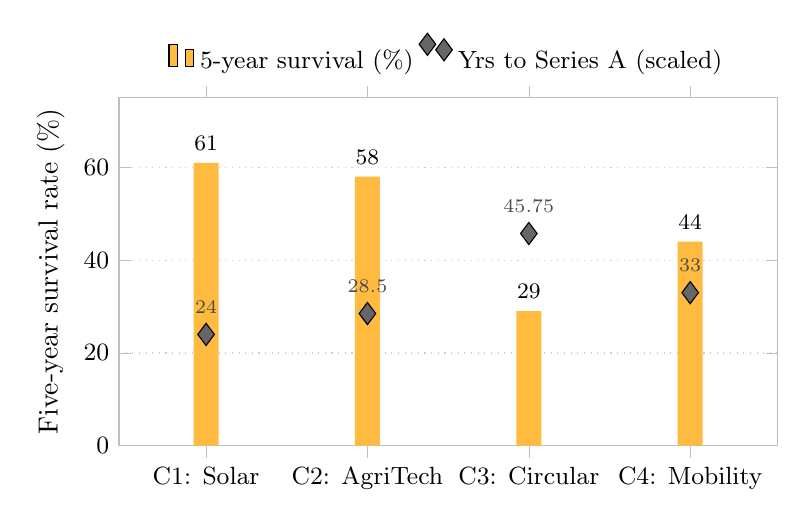
\begin{tikzpicture}
\begin{axis}[
  ybar,
  width=0.82\linewidth,
  height=6.0cm,
  bar width=9pt,
  ymin=0, ymax=75,
  ylabel={Five-year survival rate (\%)},
  symbolic x coords={C1: Solar, C2: AgriTech, C3: Circular, C4: Mobility},
  xtick=data,
  xticklabel style={font=\small},
  yticklabel style={font=\small},
  nodes near coords,
  nodes near coords style={font=\footnotesize, yshift=1pt},
  ymajorgrids=true, grid style={dotted, gray!40},
  axis line style={draw=gray!50},
  tick style={draw=gray!50},
  enlarge x limits=0.18,
  legend style={at={(0.5,1.04)}, anchor=south, legend columns=2,
                font=\small, draw=none},
]
%% Survival bars
\addplot[fill=C1Solar!75, draw=none]
  coordinates {({C1: Solar},61)({C2: AgriTech},58)({C3: Circular},29)({C4: Mobility},44)};
\addlegendentry{5-year survival (\%)}

%% Overlay axis for time-to-SeriesA (secondary axis via pgfplots trick: scale 0→10 years → 0→75%)
%% Show as dots on top
\addplot[only marks, mark=diamond*, mark size=4pt, mark options={fill=black!60},
         nodes near coords, nodes near coords align={above},
         every node near coord/.append style={yshift=3pt, font=\scriptsize, color=black!70}]
  coordinates {({C1: Solar},24.0) ({C2: AgriTech},28.5)
               ({C3: Circular},45.75) ({C4: Mobility},33.0)};
\addlegendentry{Yrs to Series~A (scaled)}
\end{axis}
\end{tikzpicture}
\caption{Five-year survival rates (bars) and median years to Series~A (diamonds, scaled) by archetype for the 794 funded ventures. Solar/Energy Access leads on both metrics; Circular/Waste ventures show critically low survival (29\%) and the longest pathway to Series~A (6.1 years), indicating structural misalignment with available finance instruments.}
\label{fig:scaling}
\end{figure}

The Solar/Energy Access cluster exhibits the strongest scaling
trajectory across all metrics: shortest median time to Series~A
(3.2 years), highest five-year survival rate (61\%), and highest
proportion reaching Series~A (22\%). These figures are consistent
with the established investment thesis and the presence of specialist
investors with deep domain knowledge who provide informed follow-on
capital. The 2015--2018 founding cohort was the most productive for
this cluster, corresponding to the period in which pay-as-you-go
solar as a category first achieved investment-grade status among DFIs
and impact investors.

The AgriTech cluster shows the strongest recent momentum: the
2019--2023 cohort is over-represented among ventures with at least
two funding rounds. Median time to Series~A (3.8 years) is only
marginally longer than the Solar cluster, though survival rates
(58\%) are somewhat lower, possibly reflecting greater business model
heterogeneity within this cluster and COVID-19 disruption to
agricultural supply chains in 2020--2021.

The Circular Economy cluster presents the most concerning trajectory:
6.1 years median to Series~A for the minority that achieve it, a
five-year survival rate of only 29\%, and a median of 1.3 funding
rounds before dormancy or exit. Only 6\% of funded Circular Economy
ventures in our sample have recorded a Series~A-equivalent round,
versus 22\% for Solar. The structural explanation is not venture
quality but financing instrument misfit: the grant-to-VC ratio of
3.7:1 indicates that these ventures draw primarily on grant capital,
but grants are project-specific, time-limited, and conditioned on
reporting milestones poorly aligned with the long lead times of
physical circular economy infrastructure development.

\subsection{Funding Stage Sequences}

Among ventures with two or more recorded funding events, we observe
distinct funding stage sequences by cluster. Solar/Energy Access
ventures most commonly follow a seed $\to$ Series~A $\to$ debt
facility sequence, with the third event typically a receivables-backed
facility from a DFI rather than an equity round. This reflects the
asset-backed nature of pay-as-you-go portfolios, in which receivables
can serve as collateral once a track record is established.

AgriTech ventures follow a grant $\to$ seed $\to$ Series~A sequence
more frequently than other clusters, with the initial grant typically
provided by AGRA, GIZ, or USAID for platform development or market
validation. This grant-to-equity conversion pattern suggests that
AgriTech ventures are using public development capital effectively
as de-risking capital that unlocks subsequent private investment---a
textbook case of blended finance additionality
\citep{reimsbach2022blended}.

Circular Economy ventures most frequently show a grant $\to$ dormancy
sequence: a single grant event followed by no subsequent recorded
funding activity. This is consistent with ventures that successfully
execute a pilot funded by a project grant but fail to convert the
pilot into a self-sustaining or investor-financeable operation.
The absence of a grant-to-equity conversion pathway distinguishes
this cluster from AgriTech and points to a missing institutional
layer: a quasi-equity instrument---revenue-based financing or
recoverable grants---calibrated to the cash flow volatility of
circular economy operations.

Mobility ventures show the most heterogeneous sequences, consistent
with the bimodal population structure identified in
Section~\ref{sec:clusters}. Urban ride-hailing ventures follow
sequences typical of VC-backed platforms (seed $\to$ Series~A $\to$
Series~B), while rural logistics ventures mirror the grant-dominated
sequences of the Circular Economy cluster.

\subsection{Geographic--Cluster Interaction Effects}

Cross-tabulating cluster membership against country reveals systematic
geographic specialisation. Kenya is disproportionately represented in
Cluster~1 (Solar/Energy Access: 35\% of KEN ventures) and Cluster~2
(AgriTech: 32\%), consistent with Kenya's mature pay-as-you-go solar
ecosystem and the concentration of agricultural SaaS platforms in
Nairobi. South Africa is strongly over-represented in Cluster~3
(Circular/Waste: 28\% of ZAF ventures), attributable to South
Africa's established recycling infrastructure, university research
programmes in materials science, and corporate sustainability
procurement commitments from large retailers. Nigeria is
disproportionately Cluster~1 and Cluster~4 (Energy Access and
Mobility), reflecting Lagos's density of consumer-facing platform
ventures and Nigeria's severe rural electrification deficit.

These geographic specialisations have practical implications for
pan-African investment mandates. A fund defining its mandate as
``African clean tech'' without geographic differentiation will in
practice concentrate in Clusters~1 and~2 in East Africa, because
that is where the most VC-legible ventures in the most investable
archetypes are concentrated. Cluster~3 ventures in Southern Africa
and Cluster~4 rural logistics ventures in Central and West Africa
will remain systematically undercapitalised unless the mandate
explicitly allocates to them.


% ===========================================================
\section{Discussion}
\label{sec:discussion}
% ===========================================================

\subsection{Policy Implications: Archetype-Differentiated Finance}

The central policy finding of this paper is that the four scaling
archetypes require fundamentally different financing instrument
designs, and that the current predominance of a small set of standard
instruments---VC equity, DFI concessional loans, bilateral grants
---fails to match the capital needs of at least two of the four
clusters (Figure~\ref{fig:finance}).

\begin{figure}[htbp]
\centering
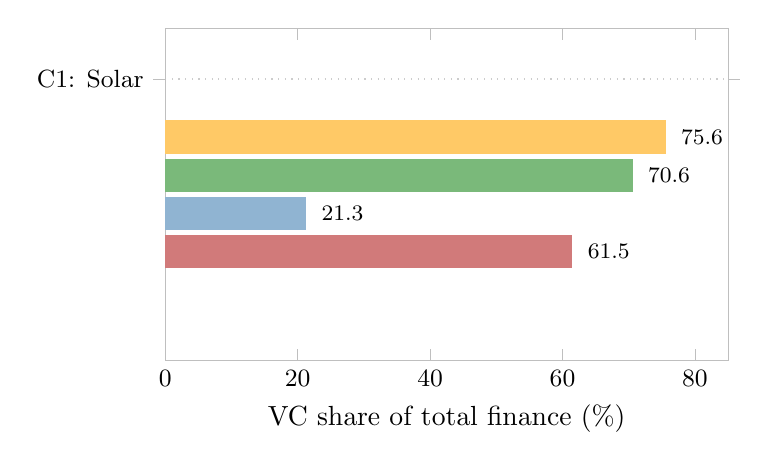
\begin{tikzpicture}
\begin{axis}[
  xbar,
  width=0.72\linewidth,
  height=5.8cm,
  bar width=12pt,
  xmin=0, xmax=85,
  xlabel={VC share of total finance (\%)},
  symbolic y coords={C4: Mobility, C3: Circular, C2: AgriTech, C1: Solar},
  ytick=data,
  yticklabel style={font=\small},
  xticklabel style={font=\small},
  nodes near coords,
  nodes near coords style={font=\footnotesize, xshift=2pt},
  nodes near coords align={horizontal},
  xtick={0,20,40,60,80},
  ymajorgrids=true, grid style={dotted, gray!40},
  axis line style={draw=gray!50},
  tick style={draw=gray!50},
  enlarge y limits=0.22,
  legend style={at={(0.5,-0.22)}, anchor=north, legend columns=2,
                font=\small, draw=none},
]
%% VC share (derived: VC / (VC + Grant) * 100)
%% C1: ratio 1:3.1 => VC=3.1, Grant=1 => VC%=75.6
%% C2: 1:2.4 => 70.6%
%% C3: 3.7:1 => 21.3%
%% C4: 1:1.6 => 61.5%
\addplot[fill=C1Solar!60, draw=none]
  coordinates {(75.6,{C1: Solar})};
\addplot[fill=C2Agri!60, draw=none]
  coordinates {(70.6,{C2: AgriTech})};
\addplot[fill=C3Circ!60, draw=none]
  coordinates {(21.3,{C3: Circular})};
\addplot[fill=C4Mob!60, draw=none]
  coordinates {(61.5,{C4: Mobility})};
\end{axis}
\end{tikzpicture}
\caption{VC share of total financing by archetype (derived from grant:VC ratios in Table~\ref{tab:cluster_profiles}). Solar and AgriTech ventures attract predominantly private capital; Circular/Waste ventures are grant-dependent (VC share of only 21\%), reflecting structural misalignment between circular economy business models and conventional VC return expectations.}
\label{fig:finance}
\end{figure}

For \textbf{Cluster~1 (Solar/Energy Access)}, the financing ecosystem
is relatively well-calibrated. Specialist investors exist, track
records are available, and DFI debt facilities have matured to support
receivables-backed portfolios. Policy priority here is
\textit{risk transfer and catalytic co-investment} at the frontier:
blended finance instruments that enable ventures to cross the gap
between Series~A and the scale at which investment-grade bond markets
become accessible \citep{lall2021scaling}. The main gap is not
instrument availability but geographic reach: pay-as-you-go finance
infrastructure is mature in Kenya but nascent in Francophone West
Africa and the DRC.

For \textbf{Cluster~2 (AgriTech Platforms)}, the grant-to-equity
conversion pathway identified in Section~\ref{sec:trajectories} is
functioning but remains fragile, depending on the presence of
sophisticated DFI investors who can bridge between grant capital and
commercial equity. Policy priority is to systematise this conversion
pathway, reducing dependence on individual investor relationships
by creating standardised milestone frameworks that allow grant-funded
AgriTech pilots to demonstrate investment readiness in a format
evaluable by multiple investors simultaneously.

For \textbf{Cluster~3 (Circular Economy/Waste)}, the financing gap
is structural and requires new instrument design. We argue for
\textit{recoverable grants}---instruments that function as grants
during the high-uncertainty pilot phase but convert to equity or
revenue-based financing if a defined revenue threshold is reached
---as the appropriate primary instrument. This structure allows
ventures to absorb the volatility of informal waste picker
coordination and commodity price fluctuations without the covenant
pressure of debt or the growth expectations of VC equity. South
Africa's blended finance ecosystem, anchored by the Industrial
Development Corporation, is best positioned to pilot such instruments
nationally, with potential for replication through the African
Development Bank's Sustainable Energy Fund for Africa.

For \textbf{Cluster~4 (Mobility/Logistics)}, the policy response
should be differentiated by the urban/rural axis identified in our
bimodal analysis. Urban mobility ventures are largely self-financing
through VC; policy priority here is regulatory (EV charging
infrastructure, ride-hailing licensing frameworks, driver welfare
standards). Rural last-mile logistics ventures need the recoverable
grant logic of Cluster~3, supplemented by procurement guarantees from
public health systems and humanitarian organisations that can anchor
revenue predictability during early scaling.

\subsection{Platform Governance Implications}

Beyond finance, the four archetypes have distinct implications for how
innovation platform operators---accelerators, corporate innovation
hubs, national innovation agencies---should design their programmes.

Clusters~1 and~2 ventures benefit most from
\textit{investor-readiness} programming: standardised impact metrics
(households connected, smallholders onboarded), financial model
templates, and introductions to specialist investors. These ventures
already know their scaling pathway; what they need is friction
reduction in the investor interface.

Cluster~3 ventures need a different form of support:
\textit{market-making} for recycled materials (connecting ventures
with corporate buyers), \textit{regulatory advocacy} (formalisation
of informal waste picker status, extended producer responsibility
legislation), and \textit{R\&D co-investment} for process technology
improvements that reduce unit costs. Accelerator programmes that
treat Cluster~3 ventures with the same investor-readiness curriculum
as Cluster~1 are systematically misaligned with these needs.

Rural Cluster~4 ventures need \textit{procurement pathway
development}: structured engagement with national health ministries,
humanitarian logistics coordinators, and agricultural development
programmes to convert one-off contracts into multi-year offtake
arrangements that can underpin financing.

\subsection{Limitations}

Three limitations merit explicit acknowledgement. First,
\textbf{Crunchbase selection bias} is the most significant
methodological concern. As \citet{rodriguez2021crunchbase} document,
Crunchbase systematically over-represents VC-backed, anglophone, and
urban ventures. Our dataset of 1,847 ventures is a biased sample of
the true population of African clean tech organisations, which
includes thousands of informal cooperatives, NGO-incubated enterprises,
and community-managed utilities invisible to Crunchbase. Funding and
survival statistics should therefore be understood as describing the
\textit{Crunchbase-visible} population, not the full clean tech
ecosystem. Circular Economy ventures are particularly affected, since
the informal character of many waste management organisations makes
them systematically less likely to appear in Crunchbase.

Second, \textbf{description quality and strategic framing} vary across
ventures. Crunchbase descriptions are self-authored marketing texts
that may not accurately represent operational reality. A venture
describing itself as an ``AI-powered agritech platform'' may in
practice be an SMS-based price information service. The embedding
model captures the language used, not the operational reality. This
limitation is intrinsic to any computational study based on textual
self-presentation and should be addressed in future work through
triangulation with administrative data or qualitative case studies.

Third, \textbf{temporal instability} of cluster membership is not
addressed in this cross-sectional study. Ventures may migrate between
archetypes as they develop: an AgriTech platform that adds a waste
management service, or an energy access venture that adds mobility
financing. Longitudinal analysis using multiple Crunchbase snapshots
would be needed to track archetype trajectories over time.


% ===========================================================
\section{Conclusion}
\label{sec:conclusion}
% ===========================================================

This paper has applied sentence-transformer embeddings and $k$-means
clustering to 1,847 African clean tech ventures from the Crunchbase
Academic dataset, revealing four empirically stable scaling
archetypes: Solar/Energy Access (37\%), AgriTech Platforms (28\%),
Circular Economy/Waste (21\%), and Mobility/Logistics (14\%). These
archetypes differ substantially in funding levels, geographic
concentration, Knowledge Triangle profiles, and scaling trajectories,
and they map onto distinct financing instrument requirements.

Our core argument is that the clean tech investment ecosystem in
Africa has matured enough for Clusters~1 and~2 but remains
structurally misaligned with Cluster~3 and the rural segment of
Cluster~4. The financing gap is not primarily a matter of capital
scarcity---Africa attracted \$6.5 billion in tech venture funding in
2022 \citep{cbinsights2023africa}---but of instrument design. The
dominant instruments (VC equity, concessional DFI debt) are
calibrated to the risk-return profile of consumer-facing digital
platforms and are poorly matched to the physical, informal, and
long-cycle economics of circular and rural logistics ventures.

The methodological contribution is to demonstrate that computational
text analysis of startup descriptions in a global commercial database
can reveal venture typologies at a resolution and scale not achievable
through survey or case-study research. The \texttt{all-MiniLM-L6-v2}
embedding model achieves silhouette scores comparable to those
obtained in studies using longer and richer texts
\citep{grimmer2021machine}, and the resulting clusters pass a topical
coherence validation against LDA-derived topics. This pipeline is
replicable across other geographic contexts and thematic domains.

For policymakers and blended finance designers, we offer four targeted
recommendations. First, design energy access blended finance for
geographic reach, not sectoral innovation: the instrument toolkit is
adequate, the deployment geography is not. Second, systematise the
grant-to-equity conversion pathway for AgriTech, reducing dependence
on bespoke investor relationships. Third, develop recoverable grant
instruments specifically calibrated for Circular Economy ventures,
accepting longer time horizons and physical commodity exposure as
structural features rather than design flaws. Fourth, disaggregate
Mobility/Logistics into urban and rural mandates with separate
instrument designs and different anchor investor types.

Future research should address the Crunchbase selection bias through
triangulation with national business registries, DFI portfolios, and
household enterprise surveys. Longitudinal analysis tracking ventures
across multiple Crunchbase snapshots would allow dynamic modelling
of archetype migration and funding stage transition probabilities.
Qualitative engagement with founders across the four clusters would
provide the experiential texture that complements the structural
findings presented here.

\vspace{2em}
\noindent\textbf{Data availability.} The Crunchbase Academic dataset
is available under an Academic License from Crunchbase. Processed
outputs and analysis code are available from the corresponding author
upon request.

\noindent\textbf{Conflict of interest.} None declared.

\noindent\textbf{Acknowledgments.} The author thanks the Rotterdam
School of Management and Erasmus Research Institute of Management for
institutional support.

% ===========================================================
%% Bibliography
% ===========================================================

\bibliographystyle{elsarticle-harv}
\bibliography{references}

\end{document}
